\documentclass[a4paper,14pt]{extreport} % формат документа

\usepackage{amsmath}
\usepackage{cmap} % поиск в ПДФ
\usepackage[T2A]{fontenc} % кодировка
\usepackage[utf8]{inputenc} % кодировка исходного текста
\usepackage[english,russian]{babel} % локализация и переносы
\usepackage[left = 2cm, right = 1cm, top = 2cm, bottom = 2 cm]{geometry} % поля
\usepackage{listings}
\usepackage{graphicx} % для вставки рисунков
\usepackage{amsmath}
\usepackage{float}
\usepackage{multirow}
\graphicspath{{pictures/}}
\DeclareGraphicsExtensions{.pdf,.png,.jpg}
\newcommand{\anonsection}[1]{\section*{#1}\addcontentsline{toc}{section}{#1}}

\lstset{ %
	language=Lisp,                % Язык программирования 
	numbers=left,                   % С какой стороны нумеровать          
	frame=single,                    % Добавить рамку
}

\begin{document}
\begin{titlepage}

    \begin{table}[H]
        \centering
        \footnotesize
        \begin{tabular}{cc}
            \multirow{8}{*}{
\includegraphics[scale=0.35]{bmstu.jpg}}
            & \\
            & \\
            & \textbf{Министерство науки и высшего образования Российской Федерации} \\
            & \textbf{Федеральное государственное бюджетное образовательное учреждение} \\
            & \textbf{высшего образования} \\
            & \textbf{<<Московский государственный технический} \\
            & \textbf{университет имени Н.Э. Баумана>>} \\
            & \textbf{(МГТУ им. Н.Э. Баумана)} \\
        \end{tabular}
    \end{table}

    \vspace{-2.5cm}

    \begin{flushleft}
        \rule[-1cm]{\textwidth}{3pt}
        \rule{\textwidth}{1pt}
    \end{flushleft}

    \begin{flushleft}
        \small
        ФАКУЛЬТЕТ
        \underline{<<Информатика и системы управления>>\ \ \ \ \ \ \ 
        \ \ \ \ \ \ \ \ \ \ \ \ \ \ \ \ \ \ \ \ \ \ \ \ \ \ \ \ \ \ \ 
    \ \ \ \ \ \ \ \ \ \ \ \ \ \ \ } \\
        КАФЕДРА
        \underline{<<Программное обеспечение ЭВМ и
        информационные технологии>>
        \ \ \ \ \ \ \ \ \ \ \ \ \ \ \ \ \ \ \ \ }
    \end{flushleft}

    \vspace{2cm}

    \begin{center}
        \textbf{Лабораторная работа № 2} \\
        \vspace{0.5cm}
    \end{center}

    \vspace{4cm}

    \begin{flushleft}
        \begin{tabular}{ll}
            \textbf{Дисциплина} & Моделирование.  \\
            \textbf{Тема} & ОДУ. Задача Коши.  \\
            \\
            \textbf{Студент} & Сиденко А.Г. \\
            \textbf{Группа} & ИУ7-63Б \\
            \textbf{Оценка (баллы)} & \\
            \textbf{Преподаватель} & Градов В.М.   \\
        \end{tabular}
    \end{flushleft}

    \vspace{4cm}

   \begin{center}
        Москва, 2020 г.
    \end{center}

\end{titlepage}

\begin{enumerate}

\item Дан разрядный контур.

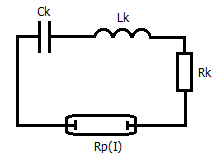
\includegraphics[scale=1]{scheme.png}

\item Получена система дифференциальных уравнений:

\begin{equation*}
    \begin{cases}
        L_\text{к}\frac{dI}{dt} + (R_\text{к} + R_p) I - U_c = 0 \\
        C_\text{к} \frac{dU_c}{dt} = -I \\
    \end{cases}
\end{equation*}

Необходимо решить систему и построить графики $I(t), U_c(t), I\cdot R_p(t), R_p(t), T_0(t)$. 

\item Cопротивление газоразрядной трубки, находится в зависимости от силы тока:

\begin{equation*}
    R_p(I) = \frac{l_{\text{э}}}{2 \pi R^2 \int_0^1 \sigma(T(z))zdz}
\end{equation*}

\item Даны 2 таблицы, для нахождения $T_0, m, \sigma$

\item Система уравнений решается методом Рунге-Кутта 4 порядка для системы ОДУ. 

\begin{equation*}
    y_{n+1} = y_n + \frac{k_1 + 2k_2 + 2k_3 + k_4}{6},
\end{equation*}

\begin{equation*}
    z_{n+1} = z_n + \frac{q_1 + 2q_2 + 2q_3 + q_4}{6}
\end{equation*}

, где

\begin{equation*}
    k_1 = h_n f(y_n, z_n), ~~q_1 = h_n \varphi (y_n)
\end{equation*}

\begin{equation*}
    k_2 = h_n f (y_n + \frac{k_1}{2}, z_n + \frac{q_1}{2}),~~ q_2 = h_n \varphi(y_n + \frac{k_1}{2})
\end{equation*}

\begin{equation*}
    k_3 = h_n f (y_n + \frac{k_2}{2}, z_n + \frac{q_2}{2}), ~~q_3 = h_n \varphi(y_n + \frac{k_2}{2})
\end{equation*}

\begin{equation*}
    k_4 = h_n f (y_n + k_3, z_n + q_3, ~~q_4 = h_n \varphi(y_n + k_3)
\end{equation*}


\begin{lstlisting}[caption=Интерполяция]
def interpolation(Y, tableY, table):
    imax = 0
    imin = 0
    for i in range(len(tableY)):
        if (Y > tableY[i]):
            imax = i
        else:
            imax = i
            break
    if (0 == imax):
        imax = 1
    imin = imax - 1

    return table[imin] + (table[imax] - table[imin]) 
    / (tableY[imax] - tableY[imin]) * (Y - tableY[imin])
\end{lstlisting}

\begin{lstlisting}[caption=Интегрирование методом трапеций]
def Fint(I, z):
    t0 = interpolation(I, tableI, tableT0)
    global gt0
    gt0 = t0
    m = interpolation(I, tableI, tableM)
    t = t0 + (tw - t0) * (z ** m)
    sigma = interpolation(I, tableI, tableSigma)

    return sigma * t * z

def iint(I):
    a = 0
    b = 1
    n = 40
    h = (b - a) / n
    s = (Fint(I, a) + Fint(I, b)) / 2
    x = 0

    for i in range(n - 1):
        x = x + h
        s = s + Fint(I, x)
    s = s * h

    return s
\end{lstlisting}

\begin{lstlisting}[caption=Нахождение сопротивления газоразрядной трубки]
def Rp(le, R, I):
    return le / (2 * pi * R * R * iint(I))
\end{lstlisting}

\begin{lstlisting}[caption=Решение системы уравнений методом Рунге-Кутта]
def f(I, U, le, R, Lk, Rk):
    global grp
    grp = Rp(le, R, fabs(I))
    return (U - (Rk + grp) * I) / Lk

def Inext(I, U, le, R, Lk, hn, Rk, Ck):
    k1 = f(I, U, le, R, Lk, Rk)
    q1 = g(I, Ck)
    k2 = f(I + hn * k1 / 2, U + hn * q1 / 2, le, R,Lk,Rk)
    q2 = g(I + hn * k1 / 2, Ck)
    k3 = f(I + hn * k2 / 2, U + hn * q2 / 2, le, R,Lk,Rk)
    q3 = g(I + hn * k2 / 2, Ck)
    k4 = f(I + hn * k3, U + hn * q3, le, R, Lk, Rk)
    q4 = g(I + hn * k3, Ck)
    return I + hn * (k1 + 2 * k2 + 2 * k3 + k4) / 6

def g(I, Ck):
    return -I / Ck

def Unext(I, U, le, R, Lk, hn, Rk, Ck):
    k1 = f(I, U, le, R, Lk, Rk)
    q1 = g(I, Ck)
    k2 = f(I + hn * k1 / 2, U + hn * q1 / 2, le, R,Lk,Rk)
    q2 = g(I + hn * k1 / 2, Ck)
    k3 = f(I + hn * k2 / 2, U + hn * q2 / 2, le, R,Lk,Rk)
    q3 = g(I + hn * k2 / 2, Ck)
    k4 = f(I + hn * k3, U + hn * q3, le, R, Lk, Rk)
    q4 = g(I + hn * k3, Ck)
    return U + hn * (q1 + 2 * q2 + 2 * q3 + q4) / 6
\end{lstlisting}

\end{enumerate}
\end{document}